\documentclass[a4paper]{article}
\usepackage{listings}
\usepackage{xcolor}
\usepackage {fontspec}
\setromanfont{Lantinghei SC Extralight}
\setmonofont{Courier New}
\XeTeXlinebreaklocale ``zh''
\XeTeXlinebreakskip = 0pt plus 1pt
\textheight = 650pt
\lstset{
	%行号
   numbers=left,
  %背景框
   framexleftmargin=10mm,
   frame=none,
   %背景色
   %backgroundcolor=\color[rgb]{1,1,0.76},
   backgroundcolor=\color[RGB]{245,245,244},
   %样式
   keywordstyle=\bf\color{blue},
   identifierstyle=\bf,
   numberstyle=\tiny,
   numberstyle=\color[RGB]{0,192,192},
   commentstyle=\it\color[RGB]{0,96,96},
   stringstyle=\rmfamily\slshape\color[RGB]{128,0,0},
   %显示空格
   showstringspaces=false
 }

\begin{document}
\title{实验报告 实验六}
\author{姓名:王钦\quad 学号:13349112\quad 班级:计科二班}
\date{}

\maketitle
\section*{ 实验目的}
\hangindent=4em \hangafter=-10{
  1. 理解系统调用的实现方法。\\
  2. 实现原型操作系统中一些基本的系统调用。\\
  3. 设计并实现一测试系统调用的用户程序,利用系统调用实现用户界面和内部功能。\\
  4.在原型操作系统上建立一个初步C语言开发环境,理解操作系统与高级语言之间的关系。\\
}
\section*{ 实验内容}
\hangindent=4em \hangafter=-10{
在实验四的基础上,进化你的原型操作系统,增加下列操作系统功能:\\
(1)参考下面的系统调用功能表,增加一些其他功能\\
系统调用表(局部设计)\\
(2)扩展MYOS内核,实现上表中的所有(包括你增加的)系统调用,并开发一个用户程序,展示这些系统调用的使用效果。\\
(3)设计一个C程序库,封闭getch(),gets(),putch(),puts(),scanf()和printf()等利用系统调用实现的细节,并参考下面程序,开发一个用户程序,测试这些函数功能。\\

{\scriptsize
\begin{lstlisting}[language={C}]
include stdio.h
main(){
   	char ch,str[80];
   	int a;
   	getch(&ch);
   	gets(str);
   	scanf(“a=%d”,&a);
  	putch(ch);
  	puts(str);
   	printint(“ch=%c, a=%d, str=%s”, ch, a, str);
}
\end{lstlisting}
}

\section*{ 实验平台}
\hangindent=4em \hangafter=-10{
  gcc+ld+nasm+Linux+vim\\
}

\section*{ 算法流程图}
\hangindent=4em \hangafter=-10{
  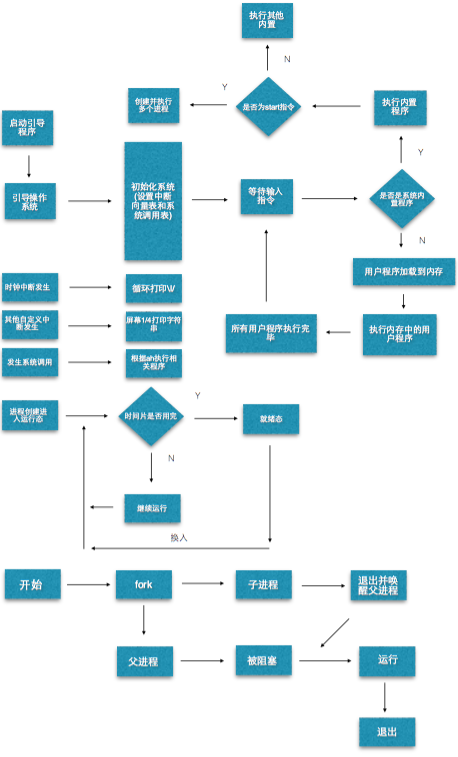
\includegraphics[scale=0.5]{Illustrations/flow.png}
}

\section*{ 功能一览}
\hangindent=4em \hangafter=-50{
	1. 系统内置功能:\\
		\indent \verb| terminal|,装载内核shell,为用户提供一个与操作系统交互的工具,开机后自动进入,以下所有功能都在terminal中交互\\
		\indent	\verb| date|, 显示当前日期\\
		\indent \verb| time|, 显示当前时间\\
		\indent \verb| asc|, 显示一个字符的asc码\\
		\indent \verb| clear|, 清除当前屏幕所有字符,刷新屏幕\\
		\indent \verb| help|, 显示系统帮助信息\\
		\indent \verb| man |, 显示内置函数的帮助信息,比如\verb| man date |,显示date的相关帮助\\
		\indent \verb| start|, 开始创建并执行四个进程并且每秒18.2次的调度,分别在屏幕\verb|1/4|处打印一些个性化信息( 不同配置的虚拟机动画速度不一样,建议使用vmware测试)\\
	2. 用户程序:\\
		\indent \verb| run |,软盘中含有三个用户程序,输入\verb|run 123|,可分别执行三个用户程序,当然也可以通过改变执行序列来改变执行的顺序\\
	3. 自定义中断:\\
		\indent 时钟中断:通过PTR每秒发出18.2次的信号来从8592芯片的RT0引脚发出终端号\verb|int 08h|来触发的用户时钟软中断\verb| int 1ch|,实现在\verb|terminal|的右下角
		一个横杠在转动.\\
		\indent 另外有自定义中断\verb|int 33h,int 34h,int 35h,int 36h|分别在屏幕四分之一的位置打印个性化信息\\
	4. 进程调度:
		\indent 软盘中共存放了用于展示进程调度的五个应用程序,其中一个应用程序为监听用户键盘事件然后退出多进程调度状态回到\verb| terminal|每个应用程序分别代表一个进程。开启装载进程并进行进程调度由\verb|1|中系统内置功能的\verb| start|指令激活。
}

\section*{ 实验步骤及效果}
\hangindent=4em \hangafter=-50{
1. 编辑修改ASM 文件,和C文件	\\\\
2. 使用make命令配合\verb|makefile|文件进行编译	\\\\
3. 运行\verb|bochs or vmware|虚拟机进行测试,进入后所看到的欢迎界面,同时进入terminal界面等待输入指令(测试多进程调度功能时请配合我提交文件中的bochsrc文件使用bochs测试,因为不同配置的虚拟机下延时动画时间不一样,我这里以我的bochs的配置为准)
{\center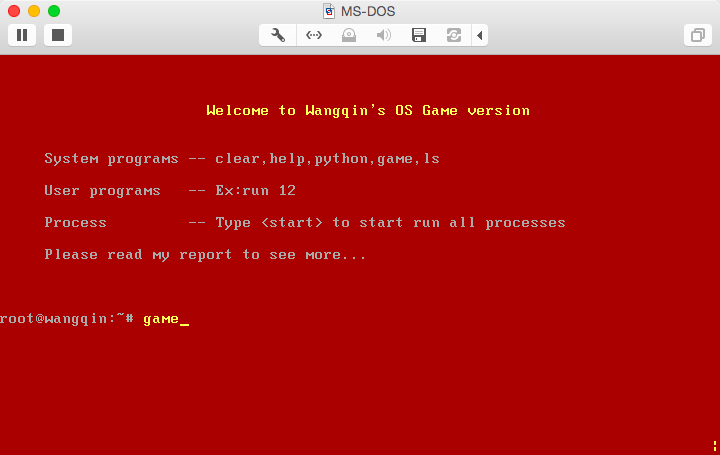
\includegraphics[scale=0.5]{Illustrations/start.png}}\\\\
4. 我们可以执行\verb|man python |\\查看\verb|python|的作用,主要功能是输入一个数学表达式然后返回表达式的结果,类似\verb|python|命令行的作用。其他类似的系统内置功能也可以使用\verb|man|命令来查看帮助信息。
但目前\verb|python|只支持加法和减法且只能有两个操作数(其实主要为了展示\verb|ah=3,4|将字符串转为数值和将数值转为字符串的系统调用效果),我这里仿照\verb|linux|系统的系统调用,设置
\verb|int 80h |为所有系统调用的入口。可以看到图中分别输入加法减法,返回计算结果。如果输入的不符合格式就会返回错误提示。最后输入\verb|exit|退出\verb|python|命令行工具。
{\center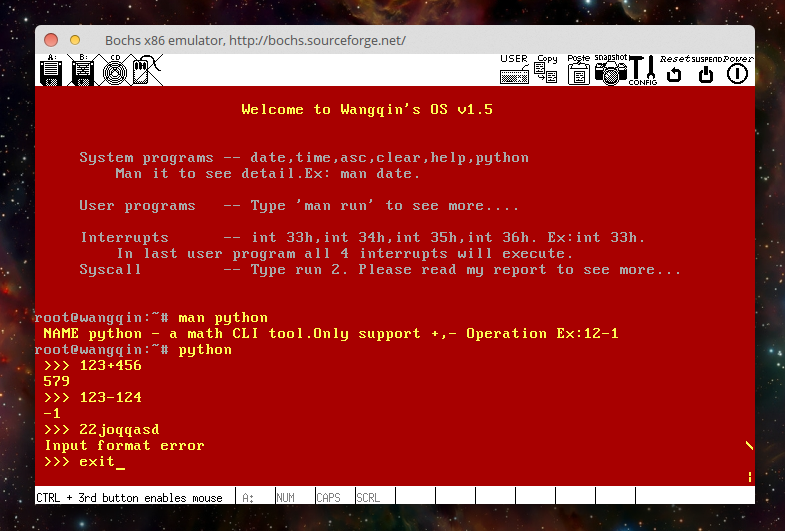
\includegraphics[scale=0.5]{Illustrations/python.png}}\\\\
5. 在terminal中输入\verb|start|命令测试多进程调度功能
6. 接下来测试ah等于\verb|0,1,2,5|的系统调用(显示\verb|OUCH|,字母大小写变化等),输入\verb| run 2 |,运行第二个用户程序,
{\center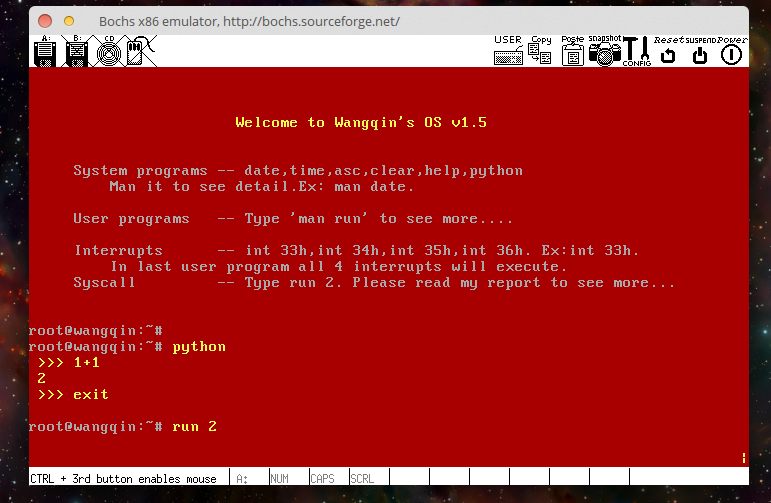
\includegraphics[scale=0.5]{Illustrations/syscall0125.png}}\\\\

下面是第二个用户程序的代码:
{\scriptsize
	\begin{lstlisting}[language={C}]
org 0x1000
;org 0x100

;#0
mov ah,0
int 80h

;LISTEN_EXIT----
listen0:
	mov ah,0
	int 16h


;#2
mov ax,0xb800
mov es,ax
mov dx,1994D
mov ah,2
int 80h

;LISTEN_EXIT----
	mov ah,0
	int 16h

;#1
mov ax,0xb800
mov es,ax
mov dx,1994D
mov ah,1
int 80h

;LISTEN_EXIT----
	mov ah,0
	int 16h



;#5
mov ax,cs
mov ds,ax
mov es,ax

mov cx,0317h  ;position
mov ah,5
mov dx,msg
int 80h


;LISTEN_EXIT----
listen:
	mov ah,0
	int 16h

ret



msg:
	db "hello world!"

times 512-($-$$) db 0	;填充剩余扇区0



	\end{lstlisting}}
下面我们将上面代码分解一下,详细介绍。\\\\
5.1 首先执行执行\verb|ah=0|的系统调用将\verb| OUCH |  打印在屏幕中间
{\scriptsize
\begin{lstlisting}[language={C}]
org 0x1000
;org 0x100

;#0
mov ah,0
int 80h
;LISTEN_EXIT----
listen0:
	mov ah,0
	int 16h

	\end{lstlisting}}
{\center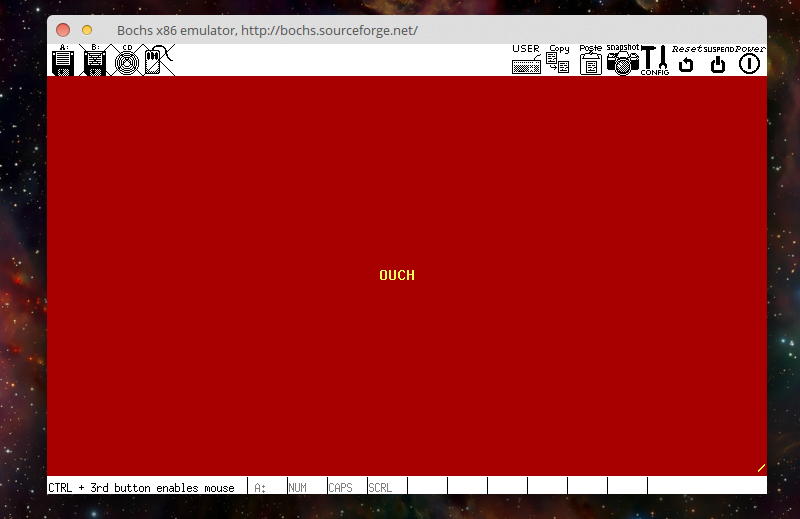
\includegraphics[scale=0.4]{Illustrations/syscall0.png}}\\\\
5.2 现在按下任意键,将执行\verb|ah=2|的系统调用把\verb| OUCH|的第一个字母大写O变成小写o\\\\
{\scriptsize
\begin{lstlisting}[language={C}]
;#2
mov ax,0xb800
mov es,ax
mov dx,1994D
mov ah,2
int 80h

;LISTEN_EXIT----
	mov ah,0
	int 16h

	\end{lstlisting}}
{\center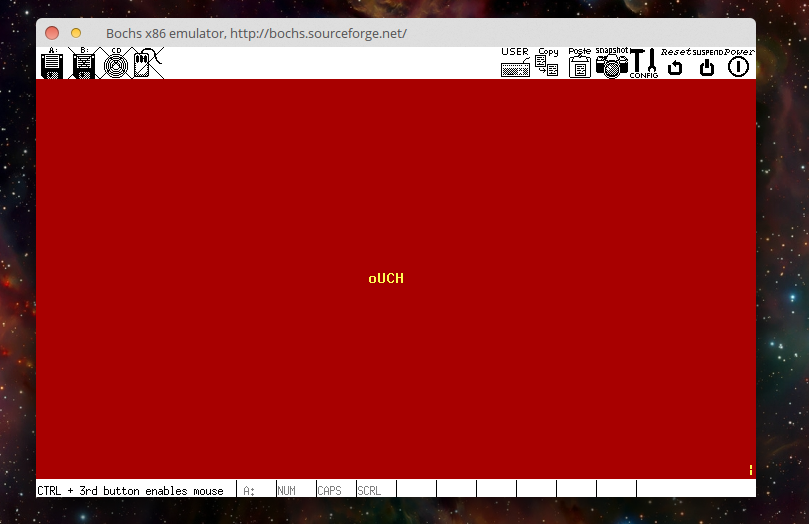
\includegraphics[scale=0.4]{Illustrations/syscall2.png}}\\\\
5.3 按下任意键,执行\verb|ah=1|的系统调用把\verb| oUCH|的第一个字母小写o变回大写O\\\\
{\scriptsize
\begin{lstlisting}[language={C}]
;#1
mov ax,0xb800
mov es,ax
mov dx,1994D
mov ah,1
int 80h

;LISTEN_EXIT----
	mov ah,0
	int 16h


	\end{lstlisting}}
{\center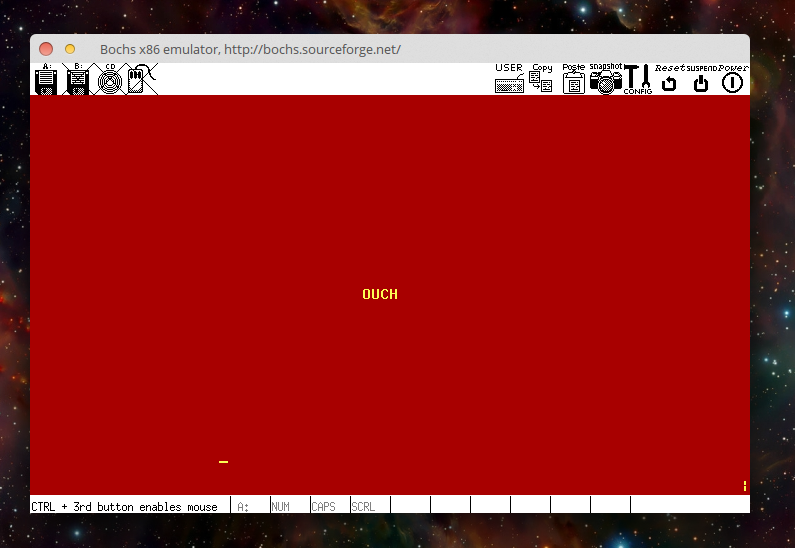
\includegraphics[scale=0.4]{Illustrations/syscall1.png}}\\\\
5.4 按下任意键,执行\verb|ah=5|的系统调用在屏幕3行17列的位置打印一个\verb|helloworld|
{\scriptsize
\begin{lstlisting}[language={C}]
;#5
mov ax,cs
mov ds,ax
mov es,ax

mov cx,0317h  ;position
mov ah,5
mov dx,msg
int 80h


;LISTEN_EXIT----
listen:
	mov ah,0
	int 16h

ret

msg:
	db "hello world!"
	\end{lstlisting}}

{\center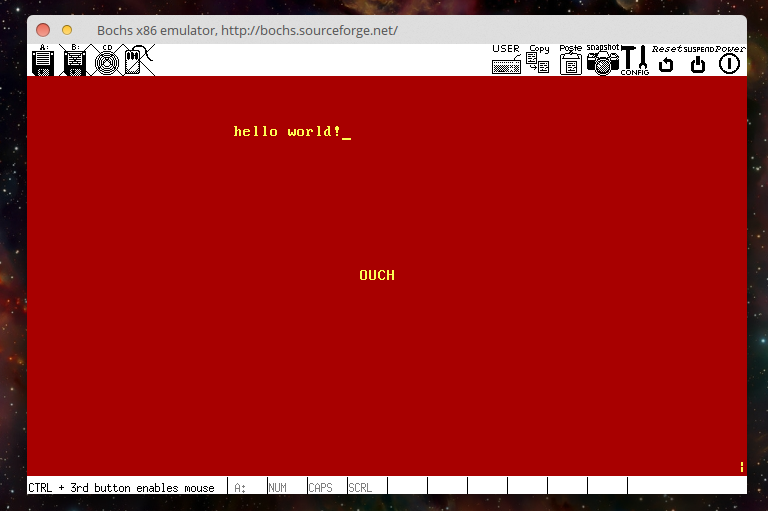
\includegraphics[scale=0.4]{Illustrations/syscall5.png}}\\\\
5.5 返回操作系统\\\\
6. 接下来我们测试封装的osclib\_share.c库里面实验所要求的\\
\verb|getch,gets,scanf,putch,putch,printint| ,输入\verb|run 1|执行第一个用户程序\\
代码如下:\\
{\scriptsize\begin{lstlisting}[language={C}]
void main(){
	screen_init();
	getch( &ch);
	gets( key);
	putch('\r');
	putch('\n');
	scanf("a=%d",&a);

	putch( ch);
	puts( key);
	printint( "ch=%c,a=%d,str=%s",ch,a,key);

	wait_key();
}

\end{lstlisting}}
6.1 首先程序等待输入一个字符
{\center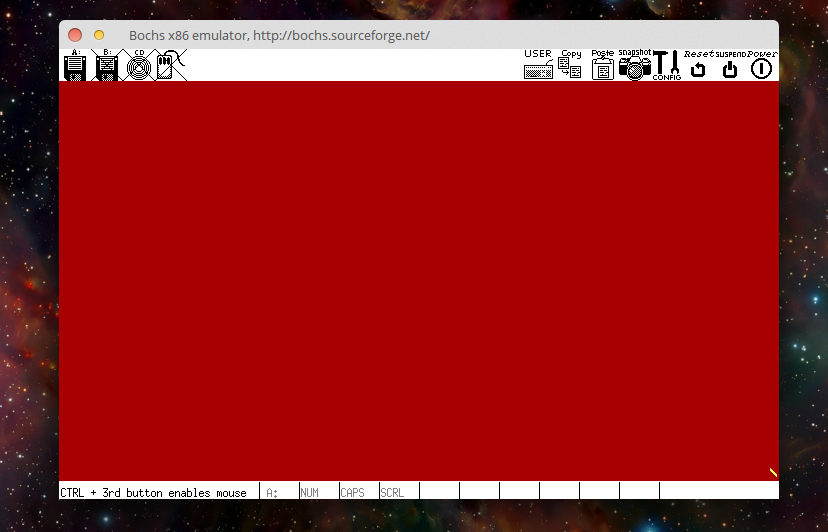
\includegraphics[scale=0.4]{Illustrations/usr1_wait.png}}\\\\
6.2 输入字符 C,回车再输入一个字符串\verb|I am a string|回车
{\center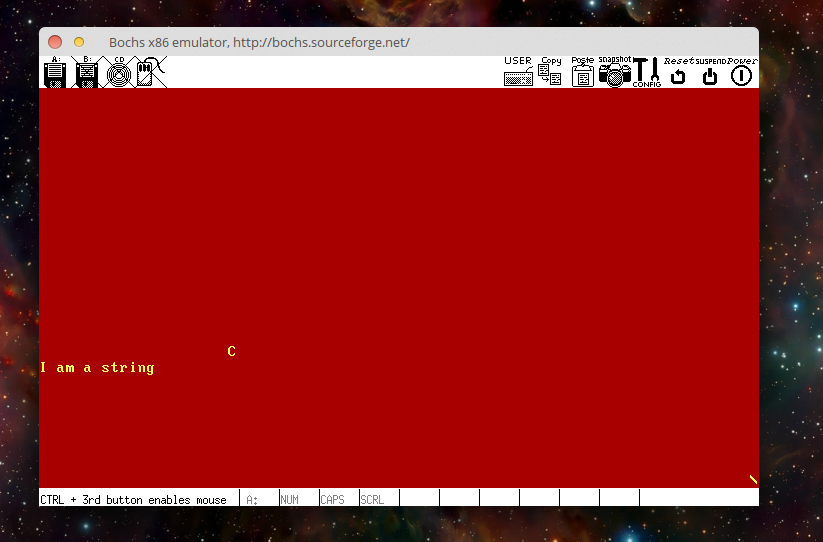
\includegraphics[scale=0.4]{Illustrations/usr1_inputstr.png}}\\\\
6.3 再输入一个int类型的数字16,回车后执行下面代码\\
{\scriptsize\begin{lstlisting}[language={C}]
	putch( ch);
	puts( key);
	printint( "ch=%c,a=%d,str=%s",ch,a,key);
\end{lstlisting}}
可以看到相继打印出了之前输入的内容
{\center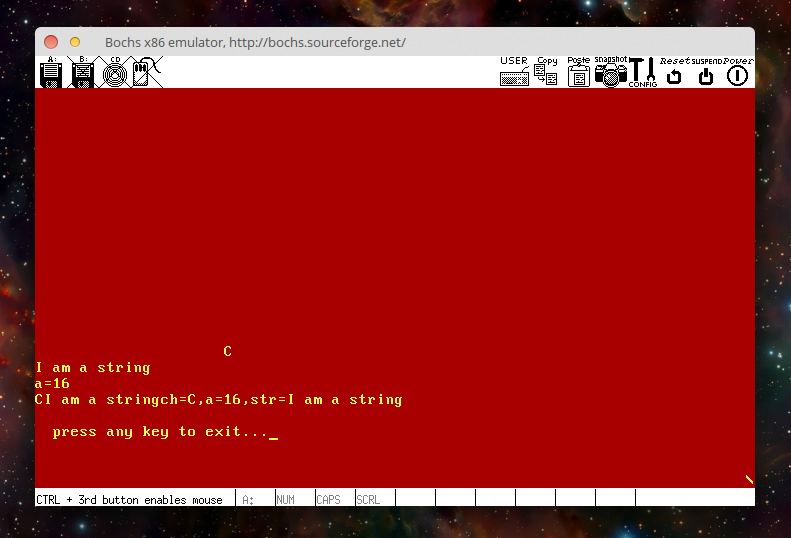
\includegraphics[scale=0.4]{Illustrations/usr1_over.png}}\\\\

7. 和之前的实验一样,内核也有设置中断,系统内置程序和重复运行多个用户程序,这里就不再赘述了。
{\center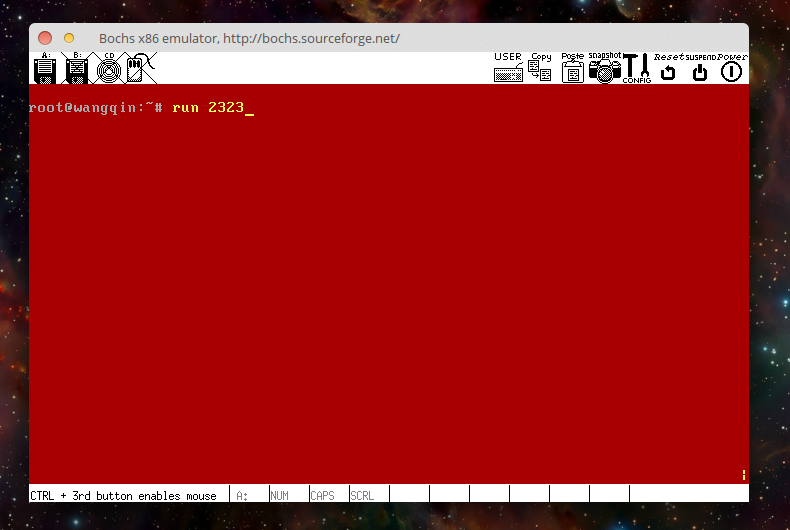
\includegraphics[scale=0.4]{Illustrations/runseq.png}}\\\\
{\center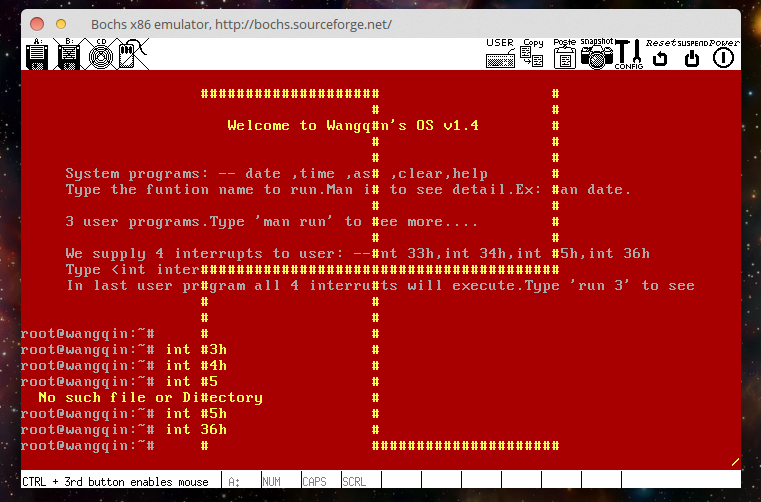
\includegraphics[scale=0.4]{Illustrations/allcustomint.png}}\\\\
{\center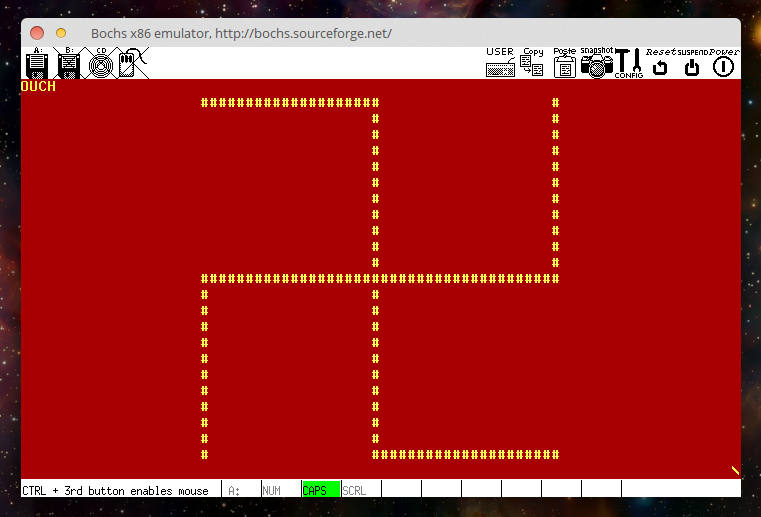
\includegraphics[scale=0.4]{Illustrations/usr3.png}}\\\\

\section*{ 内存和软盘存储管理}
\hangindent=4em \hangafter=-50{
1. 引导程序加载到内存0x7c00处运行\\
2. 引导程序将操作系统加载到0x7e00处运行\\
3. 操作系统讲用户程序加载到0x1000处运行\\
4. 软盘第1个柱面的第一个扇区存储操作系统引导程序\\
5. 软盘第1个柱面剩下所有扇区2~36扇区存储操作系统内核\\
6. 软盘第\verb|2,3,4|柱面分别存储三个用户程序\\
更多细节信息请阅读我的Makefile文件
}
\section*{ 主要函数模块解释}
\hangindent=4em \hangafter=-50{
	内核架构解释:\\
	\verb|os.c|为内核主要控制模块\\
	\verb|osclib.c os.asm|主要为\verb|os.c|提供函数实现.\\
	\verb|oslib.asm| 为\verb|osclib.c|提供更底层的函数封装\\
	\verb|osclib_share.c,oslib_share.asm| 为用户程序中所需要用到的函数,从\verb|osclib.c oslib.asm|中取出一部分作为内核和用户的共享库(使用户程序体积减少)。\\
	\verb|os_syscall.asm| 初始化系统调用和设置系统调用相关模块\\
	更多细节信息请阅读我的Makefile文件\\\\

	1. \verb|os.c: main| 函数模块,这个在之前报告中已经解释这里就不在赘述
{\scriptsize\begin{lstlisting}[language={C}]
void main(){
	//--------------------init
	init_ss();
	screen_init();
	interrupt_init();
	syscall_init();
	print_welcome_msg();
	print_message();
	print_flag(); //root@wangqin4377@:   position
	//--------------------init_end

	while(1){
		char length = listen_key();
		if_screen_scroll(); //bottom of screen
		flag_scroll();//move flag to next line
		print_flag();
	}
}
 \end{lstlisting}}
	2. 本次试验主要为了实现系统调用的工作,故在 os.asm中实现了下列函数供设置系统调用使用
{\scriptsize
	\begin{lstlisting}[language={C}]
	;---PARAM: ah is syscall num   ebx is address of syscall  bx:temp cx:function ax:sysnum
	setting_up_syscall:
	mov bx,0
	mov es,bx
	mov al,ah
	mov ah,0
	shl al,2
	mov bx,0xfe00
	add bx,ax
	mov [es:bx],ecx
	ret
	\end{lstlisting}}
	3. 初始化设置系统调用,设置全部6个系统调用功能,调用上面的函数实现

{\scriptsize
	\begin{lstlisting}[language={C}]
syscall_init:

;----#0 syscall
mov ah,0
mov ecx,0
mov cx,display_center_ouch
call setting_up_syscall

;----#1 syscall
mov ah,1
mov ecx,0
mov cx,letter_upper
call setting_up_syscall

;----#2 syscall
mov ah,2
mov ecx,0
mov cx,letter_lower
call setting_up_syscall

;----#3 syscall
mov ah,3
mov ecx,0
mov cx,atoi_syscall
call setting_up_syscall

;----#4 syscall
mov ah,4
mov ecx,0
mov cx,itoa_syscall
call setting_up_syscall

;----#5 syscall
mov ah,5
mov ecx,0
mov cx,display_str
call setting_up_syscall
ret
	\end{lstlisting}}
	4. 对\verb|scanf,printint,gets..|等函数的封装:
	其实这些函数在之前的实验中已经实现,只是名字不一样罢了。本次实验单独抽出来相关代码放在osclib\_share.c中。
	{\scriptsize
	\begin{lstlisting}[language={C}]
	\end{lstlisting}}
	5. python命令行工具:存放在\verb|python_extension.c|中,主要功能的就是使用系统调用实现字符串和数值之间的转换。
	\begin{lstlisting}[language={C}]
	unsigned short int itoa_temp;
	char * itoa_ans;
	char * itoa( short int x){
		itoa_temp = x;
		__asm__("mov $4,%ah");  // syscall num
		__asm__("push %bp");
		__asm__("int $0x80");	// syscall
		__asm__("pop %bp");
		return itoa_ans;
	}

	char *atoi_temp;
	unsigned short int atoi_ans;
	unsigned short int atoi( char * str){
		atoi_temp = str;
		__asm__("mov $3,%ah");  // syscall num
		__asm__("int $0x80");	//syscall
		return atoi_ans;
	}
	\end{lstlisting}
}

\section*{ 实验心得及仍需改进之处}
\hangindent=4em \hangafter=-50{
    实验心得:\\\\
	\indent	本次实验过程中遇到了很多挫折,最大的一个问题就是编写进程调度的算法的时候由于自己疏忽在创建进程启动进程调度的时候没有把时钟中断清零导致,无法发生下一次时钟中断,原本以为 \verb|0x1c|用户时钟中断可以不需要像\verb|0x08|那样每次对8259芯片进行重新设置。时钟中断正常工作后又发现调度出现一些问题,比如第一个进程的时间片用完之后不能换到第二个进程执行,当然这个问题还是经过调试很容易解决的。后来发现第二个进程执行用完时间片后切换到第一个进程时第一个进程无法按照原来停止执行的\verb|cs:ip|处进行执行,这个问题经过调试也是比较容易解决的。最难调试的问题是栈的切换,我这里为每个进程都设置了一个应用程序栈,进程时间片用完之后切换进程的时候进程的上下文数据RSS中
	也会包含这个进程所对应的用户程序栈的栈指针。也就是切换进程的时候也要对应用程序栈\verb| ss:sp|进行切换,但是c语言调用汇编的时候是向栈里压两个字,而汇编返回c调用处的时候是从栈里弹出一个字到\verb| IP|指令指针寄存器。这种不对称的出栈入栈很容易造成使用栈的过程中导致栈数据混乱。而且当时钟中断的处理程序即进程调度程序执行完毕后要从栈里弹出三个字的数据到\verb| IP,CS,Flags|这些寄存器,调度的时候就要手动的先把原来的\verb| IP,cs,flags|弹出来保存然后压入新进程的\verb| ip,cs,flags|,所以保持栈清晰,有规律是非常重要的,否则进程调度将会失败。栈切换这里这里调了很长时间,得到的教训就是一定要注意细节,c调用汇编或汇编调用c都要特别注意有没有冗余的数据被压栈,注意一定要先保存\verb| ip,cs,flags,sp|和一些段寄存器的数据,合适的时机再切换栈指针寄存器。当换一个新进程开始执行的时候一定要保证这个进程上次被换下来的时候,栈指针寄存器\verb| sp|一定是上次的位置减去三个字,因为要压入\verb| ip,cs,flags|。总之注意写代码的时候注意细节总会可以大大降低debug的时间从而减少写代码的总时间,提高编程效率。同时也是
	作为一个专业学生好的习惯。这次实验中我优化了操作系统和内核的结构,将\verb| shell|和内核分开,使主内核文件\verb| os.c|代码量大大减少,向Linux提倡的微内核走进了一步。
	实验仍需改进之处:\\\\
	仍需完善细节,比如说python的命令行工具加入乘法,除法完全是几行代码的问题\\
	可以考虑将用户程序做成elf格式,动态链接系统的代码库。目前的情况是用户程序自己带着一份和操作系统一样的代码库,分别联合编译\\
	考虑精简操作系统代码,减少冗余代码\\
	继续优化调整内核架构和内存磁盘管理\\
}

\end{document}
